\section{Results}
\label{sec:results}

Section~\ref{sec:devres} summarises development, Section~\ref{sec:history} the first confirmation and why the method changed, and Sections~\ref{sec:confres} to~\ref{sec:integrity} the single run of the second confirmation on the 35 sealed sites. Values are given at $Q = 6$ under independent loss with loss probability 0.3 unless stated, and all confirmation values are at byte level.

\subsection{Development results}
\label{sec:devres}
On the 2023 development data, the findings that shaped the method were the following (slot model unless stated):
\begin{itemize}
  \item Soundness: no certificate design gave a wrong decision in any condition.
  \item Witnesses added decisions: a witness placed inside the record code did almost nothing for the 7DADM, which needs seven informative days; placement in a protected group mattered.
  \item Targeting paid: against the same layering on random days, the targeted rule gained 0.10 to 0.15 on near 7DADM windows and 0.17 on hard conductance days.
  \item The exact allocator did not beat the simple rule on hard cases; the simple rule was within 7\% (at $Q = 6$) and 1.6\% (at $Q = 12$) of the optimum of the stated objective.
  \item Send-on-delta needed 1.79 times as many values as the piecewise-linear record, and a tightened tolerance did not improve hard-case decisions at this quota.
  \item With the flags allowed to use the record, hosting all witnesses in the spare room of the flag design (hybrid 1) added only 0.02 to 0.03 on unconfigured thresholds, and adding the 3b rule to the flags (hybrid 2) lost 0.16 to 0.19 of record recovery against the record alone at $Q = 6$. Of the layered designs, only the 3b rule met the adoption rule written before the run (a gain of at least 0.10 over the fair comparator in all four conditions, and a record cost of at most 0.08 against the record alone).
  \item Moving from CRC-16 to CRC-24 cost one record value per message. On the CRC-24 frame the 3b rule's record cost at $Q = 6$ was 0.088 (independent loss) at byte level, beyond the 0.08 of the adoption rule. The 3b rule was adopted nevertheless. An earlier justification, that the cost was small against the fair comparator, rested on the modelling error described in Section~\ref{sec:history} and was withdrawn; the adoption is therefore post hoc, and its cost became hypothesis H4.
\end{itemize}

\subsection{The first confirmation and the revision of the method}
\label{sec:history}
Version 2 of the method (CRC-16 frame, slot-model comparisons, nine hypotheses) was confirmed once on 31 sealed sites of 2024. Eight hypotheses held, including no wrong decision in 30,285 byte-level round trips and a gain of the 3b rule over the record alone. The integrity hypothesis failed: after one forged message that passed the CRC-16, the upper bounds of the share of days with a false certificate exceeded their limits at $Q = 12$ (0.0134 against 0.01 for the record alone and 0.0215 against 0.02 for layered witnesses). An internal review then found that the flags comparator of that study discarded the recovered record, which made the contrast against flags unfair, that several hypotheses held by construction, and that the receiver caught only some error types. These findings led to version 3: a CRC-24 per message, a hardened receiver, a flags comparator that uses the record, comparisons at byte level, and a new sealed cohort. The full results of the first confirmation are in \ref{app:confirm3} (Table~\ref{tab:confirm3}).

A second internal reading, of the version 3 plan before its freeze, found that the slot model had charged the flags one value slot per message, as on the CRC-16 frame, although the CRC-24 record symbol has 16 spare bits that hold the four flag bits. With the flags modelled correctly, the flags-plus-record design recovers the record exactly as often as the record alone. The draft's hypothesis on the record cost against that comparator was therefore dropped, the comparisons were moved to byte level with paired loss draws, and both rehearsals were repeated before the freeze. The error had no effect on the benefit hypotheses, which stayed above their limits on both development years (Table~\ref{tab:years}).

\subsection{Second confirmation: the three tests held}
\label{sec:confres}
Table~\ref{tab:hyp} lists every hypothesis with its type, limit, result, and outcome. All three tests held, the two code checks passed, and the known limit replicated (Fig.~\ref{fig:forest}).
\begin{itemize}
  \item H2, benefit over the fair comparator: on thresholds that the encoder did not know, the 3b rule decided 0.226 (0.196 to 0.258) more hard cases than flags plus record at $Q = 6$ under independent loss and 0.189 (0.165 to 0.215) under Gilbert loss; at $Q = 12$, 0.182 (0.154 to 0.214) and 0.191 (0.164 to 0.222). The smallest lower bound was 0.054 above the limit of 0.10.
  \item H3, benefit over the record alone: 0.275 (0.233 to 0.324), 0.249 (0.212 to 0.292), 0.197 (0.160 to 0.246), and 0.217 (0.181 to 0.263).
  \item H4, the cost of the adopted design: the 3b rule recovered the whole record less often than the record alone, by 0.082 (0.064 to 0.099) and 0.068 (0.055 to 0.081) at $Q = 6$, and by 0.026 (0.017 to 0.035) and 0.032 (0.023 to 0.041) at $Q = 12$. The lower bounds were within the limits of 0.15 and 0.10. The point cost at $Q = 6$ under independent loss, 0.082, was again beyond the 0.08 of the original adoption rule; H4 shows that the cost is bounded, not that the adoption rule was met.
  \item H1, soundness: no certain decision was wrong in any design, plan, or loss model, no decoded value differed from the plan, no decision-layer error occurred, and 41,668 blocks (10,417 days, two designs, two plans, all messages delivered) passed the byte-level round trip. The caveat of Section~\ref{sec:procedure} applies.
  \item H6, the known limit: at the configured thresholds the flags-plus-record design decided more hard cases than the 3b rule, by 0.028 (0.022 to 0.034) under independent loss and 0.107 (0.099 to 0.117) under Gilbert loss.
  \item H8, code check: for the record alone, the byte frame and the slot model agreed in whole-record recovery within 0.001.
\end{itemize}

\begin{figure}[t]
\centering
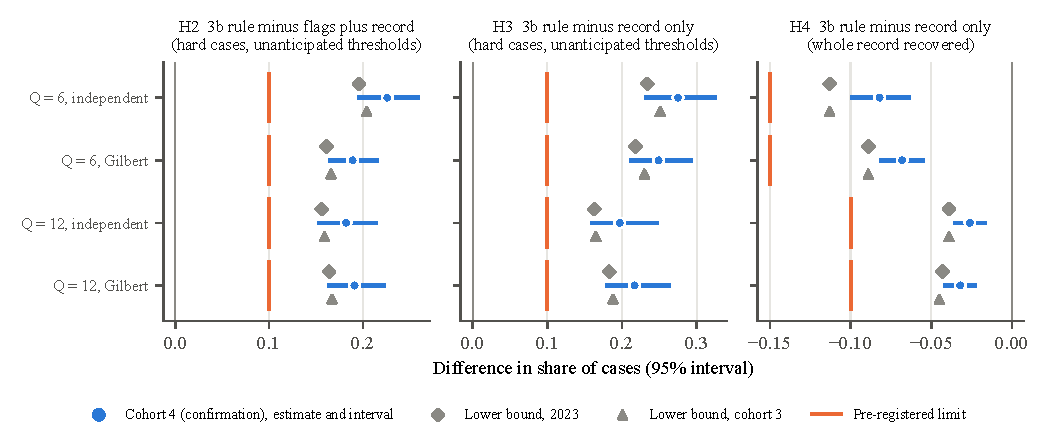
\includegraphics[width=\textwidth]{figs/forest.pdf}
\caption{The three tests on the sealed cohort with 95\% site-clustered intervals, the lower bounds of the same tests on the two development years (grey), and the pre-registered limits (orange).}
\label{fig:forest}
\end{figure}

The confirmation cohort fell within the range of the two development years on every test (Table~\ref{tab:years}). The cost was slightly smaller than in development (0.082 against 0.088 and 0.094 at $Q = 6$ under independent loss).

\begin{table}[!htbp]
\centering
\caption{The three tests on the two development years and on the confirmation cohort, computed by the same frozen code (point estimate with the lower bound of the 95\% interval in brackets; ind.\ is independent loss and Gil.\ is Gilbert loss).}
\label{tab:years}
\scriptsize
\begin{tabular}{@{}>{\raggedright\arraybackslash}p{1.9cm}>{\raggedright\arraybackslash}p{1.8cm}cccc@{}}
\toprule
Test & Year & $Q = 6$, ind. & $Q = 6$, Gil. & $Q = 12$, ind. & $Q = 12$, Gil. \\
\midrule
\tableinput{tables/years.tex}
\bottomrule
\end{tabular}
\end{table}

\subsection{Robustness of the estimates (post hoc)}
\label{sec:robust}
The confirmatory estimates were re-analysed after the run from the run's own per-site outputs; nothing was re-simulated. The conclusions did not depend on the weighting or the number of resamples:
\begin{itemize}
  \item With 10,000 resamples instead of 1,000, every interval of H2 to H4 changed by at most 0.002 at either end.
  \item With equal weight per site, the H2 contrasts were 0.178 to 0.217 (lowest lower bound 0.154) and the H3 contrasts 0.191 to 0.258 (lowest lower bound 0.159); the H4 costs were 0.025 to 0.080.
  \item With equal weight per query kind, the H2 contrasts were 0.148 to 0.209 (lowest lower bound 0.125) and the H3 contrasts 0.164 to 0.262 (lowest lower bound 0.130).
  \item Every one of the 35 sites had a positive H2 and H3 contrast in all four conditions (Fig.~\ref{fig:sites}); for H2 at $Q = 6$ under independent loss the 5th, 50th, and 95th percentiles of the site contrasts were 0.117, 0.207, and 0.361. The record cost varied more between sites: at $Q = 6$ under independent loss the 5th percentile of the site differences was $-$0.160 and the median $-$0.062.
\end{itemize}

\begin{figure}[t]
\centering
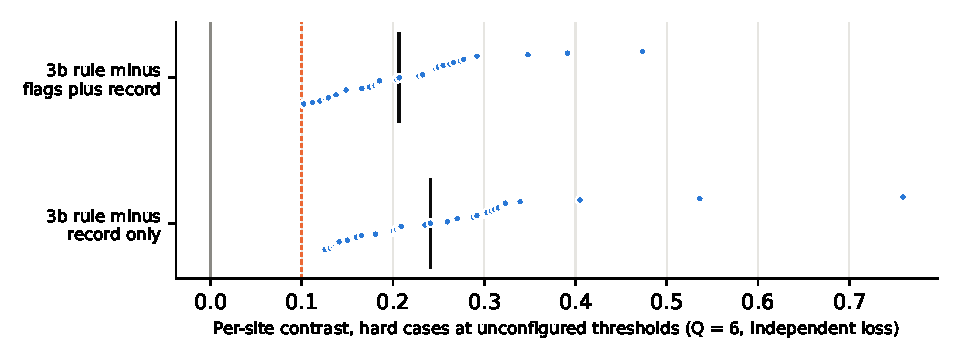
\includegraphics[width=0.9\textwidth]{figs/sites.pdf}
\caption{Per-site contrasts on the sealed cohort at six messages per day under independent loss (35 sites; the bar is the median; the dashed line is the pre-registered limit of the pooled contrast). Post hoc.}
\label{fig:sites}
\end{figure}

\subsection{Descriptive comparison}
\label{sec:desc}
Table~\ref{tab:desc} and Fig.~\ref{fig:tradeoff} show the pooled levels of the designs; these results carry no verdict.
\begin{itemize}
  \item The flags-plus-record design decided 0.999 of hard cases at configured thresholds and 0.572 at unconfigured thresholds; the 3b rule decided 0.971 and 0.798. Flags that do not use the record (slot model) decided 0.199 at unconfigured thresholds.
  \item The record alone recovered the whole record on 0.842 of days and the 3b rule on 0.760; at $Q = 12$ the figures were 0.964 and 0.937 (Table~\ref{tab:desc12}).
  \item The slot model, run as a cross-check, reproduced the byte frame within 0.001 for the record alone and the flags-plus-record design and was pessimistic for the 3b rule by 0.027 to 0.036 in whole-record recovery, because it assigns the witness group whole slots.
\end{itemize}

\begin{figure}[t]
\centering
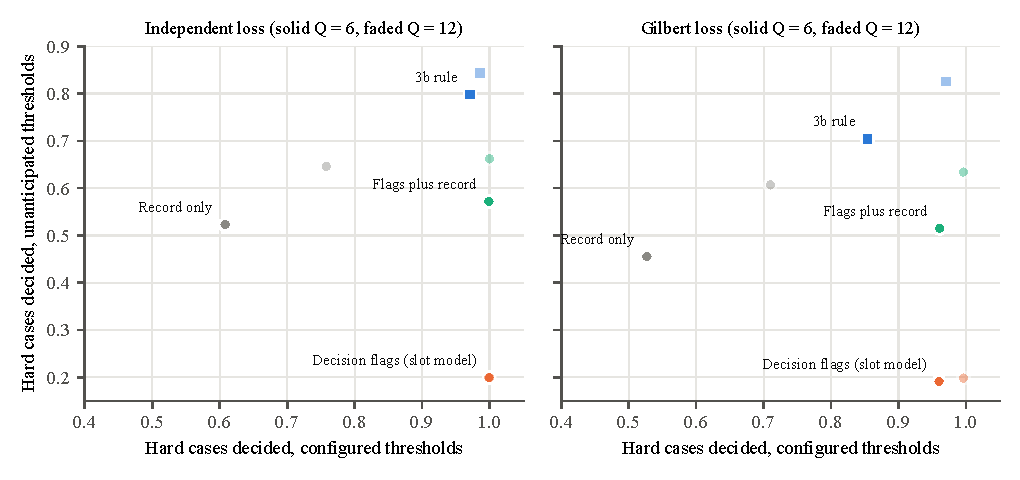
\includegraphics[width=\textwidth]{figs/tradeoff.pdf}
\caption{Hard cases decided at configured and at unconfigured thresholds on the sealed cohort (solid markers six messages per day, faded markers twelve). The flags decide almost every configured hard case; the 3b rule decides the most unconfigured ones.}
\label{fig:tradeoff}
\end{figure}

\begin{table}[!htbp]
\centering
\caption{Pooled levels at six messages per day on the sealed cohort (record recovered, hard cases at configured (conf.) thresholds, hard cases at unconfigured (unconf.) thresholds, and all days at configured thresholds).}
\label{tab:desc}
\small
\begin{tabular}{@{}lrrrr@{}}
\toprule
Design & Record & Hard, conf. & Hard, unconf. & All, conf. \\
\midrule
\tableinput{tables/confirm_desc.tex}
\bottomrule
\end{tabular}
\end{table}

\begin{table}[!htbp]
\centering
\caption{Pooled levels at twelve messages per day (same columns as Table~\ref{tab:desc}).}
\label{tab:desc12}
\small
\begin{tabular}{@{}lrrrr@{}}
\toprule
Design & Record & Hard, conf. & Hard, unconf. & All, conf. \\
\midrule
\tableinput{tables/confirm_desc12.tex}
\bottomrule
\end{tabular}
\end{table}

Table~\ref{tab:kinds} splits the contrasts by query kind, because the pooled hypotheses weight each kind by its number of hard cases.
\begin{itemize}
  \item At unconfigured thresholds the 3b rule exceeded the flags-plus-record design for every kind under both loss models, with every interval above zero: by 0.106 (pH) to 0.311 (conductance change) under independent loss. No single kind drove the pooled result.
  \item At configured thresholds the flags-plus-record design exceeded the 3b rule for every kind. The largest gap was for the 7DADM under Gilbert loss, where a seven-day window needs an informative day in each of seven blocks and a burst of losses removes the witnesses that the flags do not need.
\end{itemize}

\begin{table}[!htbp]
\centering
\caption{Contrasts at six messages per day by query kind, with 95\% site-clustered intervals: the 3b rule minus flags plus record (F+R) and minus the record alone at unconfigured (unconf.) thresholds, and the 3b rule minus F+R at configured (conf.) thresholds.}
\label{tab:kinds}
\scriptsize
\begin{tabular}{@{}lccc@{}}
\toprule
Kind & 3b $-$ F+R, unconf. & 3b $-$ record, unconf. & 3b $-$ F+R, conf. \\
\midrule
\tableinput{tables/confirm_kinds.tex}
\bottomrule
\end{tabular}
\end{table}

Table~\ref{tab:region} splits the levels by region. The regions have one to five sites; therefore, the figures carry no interval and no verdict. The 3b rule decided the most unconfigured hard cases in every region. Its record cost relative to the record alone ranged from 0.015 in the Gulf and lower Mississippi region (two sites, where the record alone recovered 0.988 of days) to 0.129 in the Mid-Atlantic and Appalachia region (independent loss).

\begin{table}[!htbp]
\centering
\caption{Levels at six messages per day by region (hard cases decided at unconfigured thresholds, then record recovered, separated by a bar; number of sites in brackets; descriptive).}
\label{tab:region}
\footnotesize
\begin{tabular}{@{}lccc@{}}
\toprule
Region & Record only & 3b rule & Flags plus record \\
\midrule
\tableinput{tables/confirm_region.tex}
\bottomrule
\end{tabular}
\end{table}

\subsection{Integrity under a forged message}
\label{sec:integrity}
The integrity study forced one arrived message per day to be forged: one to three bytes of its header or body were changed at random and its CRC-24 was recomputed; the receiver therefore accepted it as valid. Its results are descriptive (Table~\ref{tab:integrity}); the corresponding hypothesis H7 is an analytic bound.
\begin{itemize}
  \item The receiver rejected the block in 0.80 of forged days at $Q = 6$ and 0.91 at $Q = 12$.
  \item False certificates (a reading certified outside its tolerance, or a witness code that differs from the truth) occurred only on days on which no redundant message arrived: exactly the needed number of messages (a false share of 0.16 to 0.22 on such days), fewer than needed, or uncoded oversize days. With more messages than needed the share was 0.000, as corroboration predicts.
  \item A wrong decision on the day followed a forgery on 0.019 (record only) and 0.022 (3b rule) of forged days at $Q = 6$, and on 0.002 at $Q = 12$. No decision-layer error occurred.
  \item Multiplied by the probability that a corrupted message passes the CRC-24 at the assumed bit-error rate of $10^{-3}$, the expected number of days with a false certificate was at most 0.0035 per million days (upper bound, 3b rule, $Q = 6$); the ceiling for any receiver is 0.042 at $Q = 6$ and 0.084 at $Q = 12$.
\end{itemize}

\begin{table}[!htbp]
\centering
\caption{Integrity given one forged message that passes the CRC-24 (shares of forged days): block rejected; false-certificate share by class of day (more, exactly, or fewer messages than needed, and uncoded oversize days); and days with a wrong decision with their 95\% interval.}
\label{tab:integrity}
\scriptsize
\begin{tabular}{@{}lccccccc@{}}
\toprule
Design & $Q$ & Rejected & More & Exactly & Fewer & Uncoded & Wrong decision \\
\midrule
\tableinput{tables/confirm_integrity.tex}
\bottomrule
\end{tabular}
\end{table}

\subsection{Exploratory analyses after the confirmation (post hoc)}
\label{sec:explore}
The analyses in this subsection were run after the confirmation, and none of them is a test. They reuse the frozen decoder and decision code at byte level, with loss draws shared by the three designs, and were run on the two development years first and on the sealed cohort second. Values are for the sealed cohort at six messages per day under independent loss 0.3 unless stated; the full tables are in \ref{app:explore} (Tables~\ref{tab:exploss}, \ref{tab:exputil}, \ref{tab:expr}, and \ref{tab:expbase}). No certain decision was wrong in any of these runs, except where a wrong reporting resolution was imposed on purpose. A first version of the threshold sweep reported 215 wrong 7DADM decisions at 22\,\textdegree C on one development site; they came from the evaluation itself, which compared a seven-day mean that is exactly 22.0 in decimal arithmetic but 22.000000000000004 in floating point, and the certificate was right. Computed quantities are now rounded before the truth is evaluated.

Threshold sweep: Fig.~\ref{fig:thresholds} shows the share of hard cases decided correctly as the threshold moves away from the configured one, with a hard case defined at each threshold by the bands of the study. The flags-plus-record design decided 0.999 of hard cases at each configured threshold and fell to the level of the record alone beside it, because a configured answer implies little about another threshold. The 3b rule degraded in one direction only. Toward more extreme thresholds it stayed high: dissolved oxygen below 2 to 4.5\,mg/L 0.934 to 0.984, pH below 6.0 and 6.3 about 0.93, pH above 9.2 and 9.5 0.986 and 0.993, and a conductance change above 20\% and 30\% 0.980 and 0.986 (record alone 0.46 to 0.70). Toward less extreme thresholds it fell to the level of the other designs: dissolved oxygen below 6 and 7\,mg/L 0.740 and 0.745 (record alone 0.687 and 0.724), pH above 8.0 0.686 (0.661), and a conductance change above 2.5\% 0.446 (0.211). The reason is the targeting rule: a day that is hard at a more extreme threshold is also near or across the configured one; therefore, its witnesses had the protected columns; a day that is hard only at a less extreme threshold was easy at the configured one, and its witnesses were only hosted. For the 7DADM, whose daily maxima are carried on hard days on either side, the 3b rule decided 0.840 to 0.954 between 18 and 22\,\textdegree C and 0.706 and 0.682 at 16 and 24\,\textdegree C. The two development years showed the same shapes (grey lines).

\begin{figure}[t]
\centering
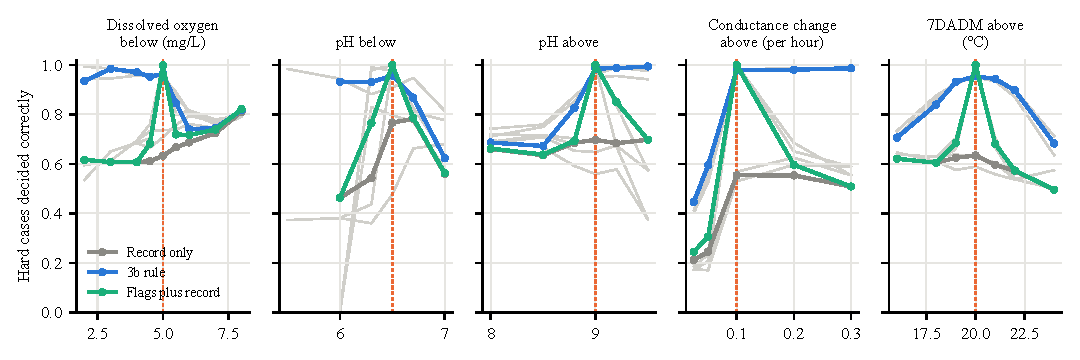
\includegraphics[width=\textwidth]{figs/thresholds.pdf}
\caption{Hard cases decided correctly as the threshold moves away from the configured one (dashed), at six messages per day under independent loss 0.3; the sealed cohort in colour, the two development years in grey. Post hoc.}
\label{fig:thresholds}
\end{figure}

Loss sweep: Across independent loss of 0.1, 0.3, and 0.5, Gilbert loss of 0.3 with mean bursts of three and six messages, and Gilbert loss of 0.5 with bursts of three, at six and twelve messages per day, the contrast of the 3b rule with flags plus record at the unconfigured thresholds of the study stayed between 0.139 and 0.248 on the three years, with every lower bound at least 0.114; the contrast with the record alone stayed between 0.174 and 0.356. Longer bursts reduced the gain most (on the cohort 0.147 at six messages per day with bursts of six, against 0.191 with bursts of three). The cost in whole-record recovery grew with loss, from 0.053 at loss 0.1 to 0.096 at loss 0.5 on the cohort (six messages per day, independent loss), and stayed at most 0.096 in every condition on the cohort.

Record utility: On days whose whole record was not recovered, a substantial part of each day was still certified within tolerance: 0.416 of the readings for the record alone and 0.429 for the 3b rule at loss 0.3, and 0.28 to 0.29 at loss 0.5. Over all days, the share of readings certified was 0.908 for the record alone and 0.862 for the 3b rule. A failed whole-record recovery is therefore not a lost day, and the cost of the witnesses in certified readings (0.046 of readings) is about half of their cost in whole-record recovery.

Assumption R: With R off, the share of correct certain decisions fell by 0.003 to 0.006 on the three years, and no decision was wrong. With a deliberately wrong resolution (ten times too coarse, or 0.1 where none had been inferred), between 24,031 and 43,247 of about 1.8 million decisions per year and design were certain but wrong (1.3\% to 2.3\%). The assumption is therefore cheap to drop and dangerous to set wrongly: in deployment the resolution must be a declared, verified field of the site profile, not a value inferred from the record, and a site without a verified resolution should run with R off.

Baselines on the final frame: coded send-on-delta and the record at half the tolerance were compared with the record alone and the 3b rule in the slot model with four value slots per message (the frame of the confirmation; send-on-delta has no byte-level frame), on the sealed cohort (Table~\ref{tab:expbase}). The slot model understates the 3b rule (by about 0.03 in whole-record recovery). Send-on-delta was the weakest design in every condition: at six messages per day under independent loss it recovered the whole record on 0.449 of days and decided 0.313 of hard cases at configured and 0.302 at unconfigured thresholds, against 0.842, 0.612, and 0.525 for the record alone. The record at half the tolerance recovered the whole record less often than the record alone in every condition (0.592 against 0.842 at six messages per day); at twelve messages per day it decided more hard cases than the record alone (0.731 against 0.647 at unconfigured thresholds, independent loss) but fewer than the 3b rule (0.820), and at six messages per day it decided fewer than the record alone. The 3b rule decided the most hard cases at both kinds of threshold in every condition (for example 0.974 and 0.777 at six messages per day), at its cost in whole-record recovery. Neither alternative way of spending the bytes reached the decisions of the 3b rule, and neither preserved the record better than the record alone.
